\section{引言}

一个记忆回答至少涉及三层证据：文档写了什么，系统如何把句子链接到实体，以及智能体实际读了哪些段落。把三者混在一起，会让看似合理的答案难以审计。假设文档写着“Alex批准了合同”，而集合中有一位实验室的Alex和一位供应商的Alex。这句话支持“发生过批准”这一说法，却不足以确定身份。后续的组织信息或关系证据可能改变链接；过早合并则可能让错误的历史看起来像权威记录。

更新事实也有同样的校准问题。一位朋友一月说“我暂时不吃辣”，六月又说“我现在可以吃辣了”。两句话都是证据；回答当前偏好时应使用后一句，而解释变化过程时则需要查看两句。因此，保留记录和解释记录需要分属不同状态。

Deep-Dream以\emph{文档优先的时间概念图}实现这种分离。文档、Episode及精确来源偏移保留原始记录；观测把抽取内容链接到原文片段，概念、关系、版本和候选族提供可修订的访问路径。新证据可以重定向链接而不改写来源。处理时间负责排列更新顺序，文档中的日期仍是观测内容。这是一种可审计的表示，并不保证实体解析正确，也不保证实现能够恢复任意历史图状态。

查询时，智能体沿地址打开来源段落，并判断证据是否充分（Figure~\ref{fig:motivation}）。它可以再次检索、检查关系邻域，或比较前后措辞。\textbf{来源门只验证来源，不验证身份或蕴含关系。}因此，来源引用不能被误当作答案正确性的证明。

\begin{figure}[h]
  \centering
  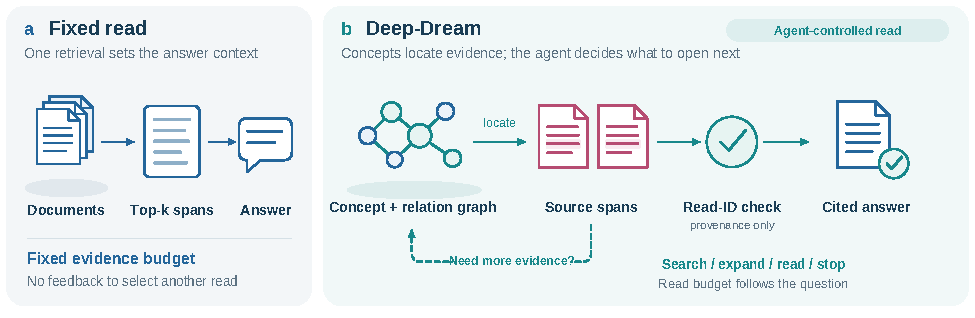
\includegraphics[width=0.98\columnwidth]{figures/fig0_motivation.pdf}
  \caption{存储与读取暴露的是不同的证据主张。可修订地址引导检索；原文段落让智能体审计措辞、身份语境和更新状态。}
  \label{fig:motivation}
\end{figure}

我们用配对构建实验、MemoryAgentBench读取路径、LongMemEval与LoCoMo历史测试，以及MEME删除检查评估两个轴。比较结果严格按协议解释：完整路径不是组件消融，同名计数只是代理指标，来源证明也不等于蕴含证明。本文贡献包括：
\begin{itemize}
    \item \textbf{校准式证据存储。} 带来源链接的观测保持可检查，推断出的身份链接可以修订。
    \item \textbf{可审计的渐进读取。} 智能体能够收集更多段落，并展示某个地址背后的证据。
    \item \textbf{双轴评估。} 在明确协议边界的前提下报告质量、覆盖、成本、对齐不确定性、图检索零结果和删除失败。
\end{itemize}
